\subsection{Max Pooling}
Max pooling is a data dimensionality reduction technique where adjacent samples are compared and only the greater one is kept.  Max pooling in general has two parameters, how many numbers are being compared (the size of the pool) and how far the pool moves between consecutive output samples.  Taking the maximum sample can be viewed as a type of non-linear filtering, the stride can be directly viewed as downsampling.  In the case of our architecture, the downsampling factor is always two, and the pool size is two as well.  Both the conceptual block diagram and the function block diagram are shown in figure \ref{fig:maxpool}

\begin{figure}[H]
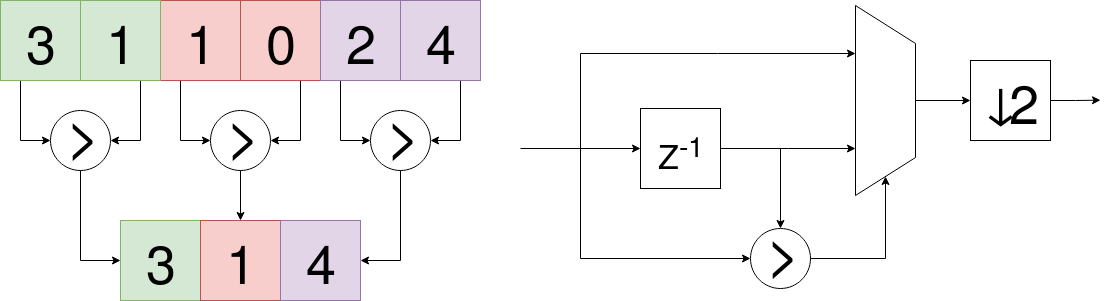
\includegraphics[width=\textwidth]{maxpool.png}
\caption{A naive/conceptual max pool (left) and a pipelined max pool (right) }
\label{fig:maxpool}
\centering
\end{figure}

The actual implementation structure of the max pooling mimics that of an FIR filter.  The difference being addition of adjacent samples has been replaced with a non-linearity, in this case a mux that choses the output based on a comparison of the two samples.  The downsampling block was implemented fairly trivially in raw VHDL.  It is essentially just a clock frequency divider, and so the data rate at all of the following stages is divided by two.  The maxpool unit was exhaustively verified by using a linear feedback shift register (LFSR) to generate every possible pair of samples possible.  The output of the hardware simulation was compared to a simple software implementation and no differences were found.
